\chapter{Theoretical Framework}

Introduction how do particles get moved get the mathematical expressions right for that 

-> Introduce Coloumb force and lorentz force 

-> Why doesn't it make sense to use the coloumb force to calculate the results (Too much data)

-> Maxwell Equations

-> Electrostatic 

-> Results in the poission equation

 exit criterion is met. This
could involve completing a preset real time, or reaching the steady state.



\begin{figure}[H]
    \centering
    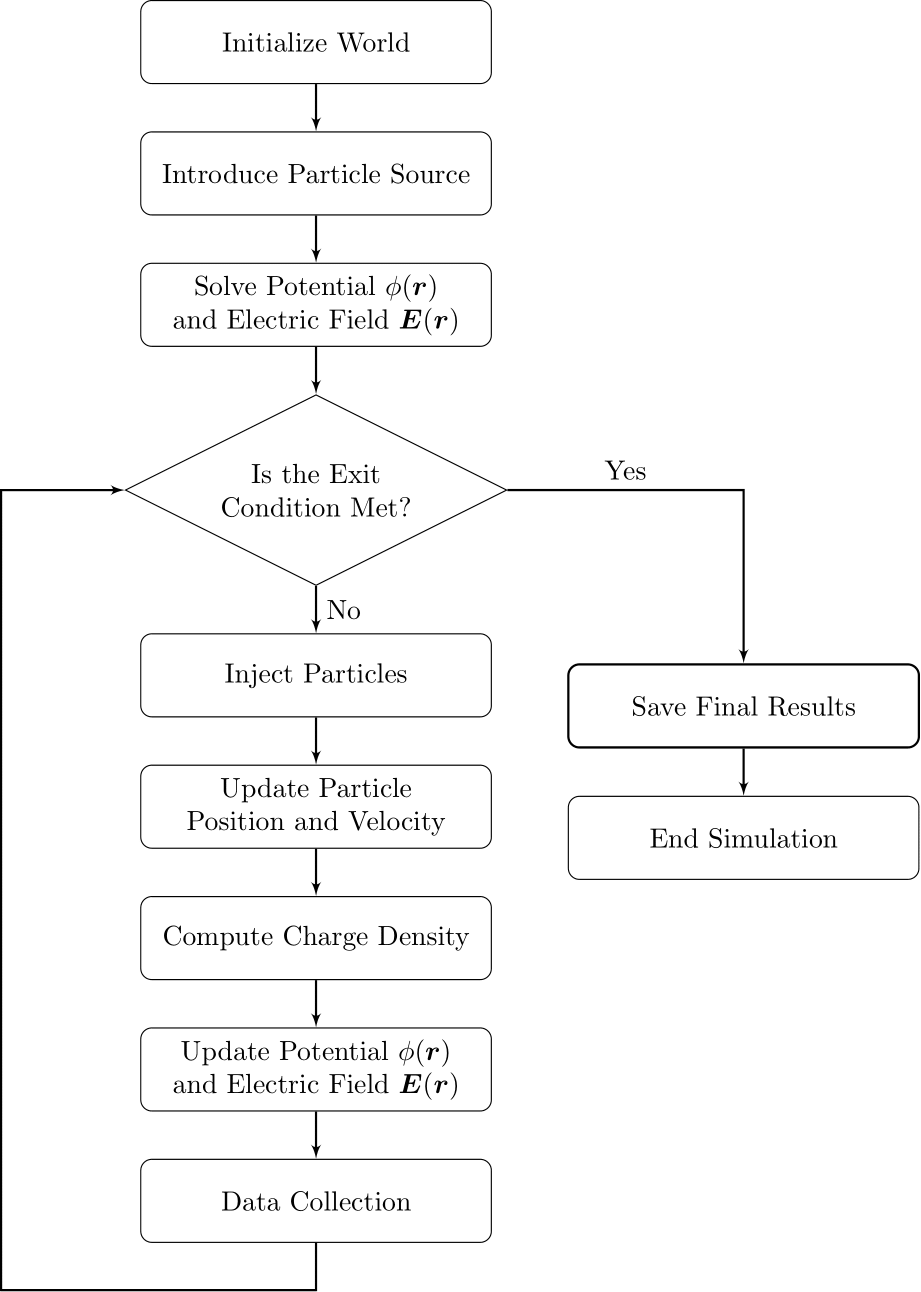
\includegraphics[width=0.7\linewidth]{figures/chapter 2/Flowchart_Studienprojekt (1).png}
    \caption{Caption}
    \label{fig:enter-label}
\end{figure}

\section{Lorentz Force}

\section{Maxwells Equations}

\subsection{Poisson Equation}

\section{Discretize World Domain}

\section{Potential Solver}

\subsection{Gauss Seidel}

\subsection{Seccesive Over Relaxation}

\section{Electric Field Solver}

\section{Particle Motion}

\subsection{Leapfrog Method}

\subsection{Interpolation}

\section{Introduction Particle Sources}

\subsection{Quiet Start method}

